\documentclass[]{book}
\usepackage{lmodern}
\usepackage{amssymb,amsmath}
\usepackage{ifxetex,ifluatex}
\usepackage{fixltx2e} % provides \textsubscript
\ifnum 0\ifxetex 1\fi\ifluatex 1\fi=0 % if pdftex
  \usepackage[T1]{fontenc}
  \usepackage[utf8]{inputenc}
\else % if luatex or xelatex
  \ifxetex
    \usepackage{mathspec}
  \else
    \usepackage{fontspec}
  \fi
  \defaultfontfeatures{Ligatures=TeX,Scale=MatchLowercase}
\fi
% use upquote if available, for straight quotes in verbatim environments
\IfFileExists{upquote.sty}{\usepackage{upquote}}{}
% use microtype if available
\IfFileExists{microtype.sty}{%
\usepackage{microtype}
\UseMicrotypeSet[protrusion]{basicmath} % disable protrusion for tt fonts
}{}
\usepackage[margin=1in]{geometry}
\usepackage{hyperref}
\hypersetup{unicode=true,
            pdftitle={A Minimal Book Example},
            pdfauthor={Yihui Xie},
            pdfborder={0 0 0},
            breaklinks=true}
\urlstyle{same}  % don't use monospace font for urls
\usepackage{natbib}
\bibliographystyle{apalike}
\usepackage{color}
\usepackage{fancyvrb}
\newcommand{\VerbBar}{|}
\newcommand{\VERB}{\Verb[commandchars=\\\{\}]}
\DefineVerbatimEnvironment{Highlighting}{Verbatim}{commandchars=\\\{\}}
% Add ',fontsize=\small' for more characters per line
\usepackage{framed}
\definecolor{shadecolor}{RGB}{248,248,248}
\newenvironment{Shaded}{\begin{snugshade}}{\end{snugshade}}
\newcommand{\KeywordTok}[1]{\textcolor[rgb]{0.13,0.29,0.53}{\textbf{#1}}}
\newcommand{\DataTypeTok}[1]{\textcolor[rgb]{0.13,0.29,0.53}{#1}}
\newcommand{\DecValTok}[1]{\textcolor[rgb]{0.00,0.00,0.81}{#1}}
\newcommand{\BaseNTok}[1]{\textcolor[rgb]{0.00,0.00,0.81}{#1}}
\newcommand{\FloatTok}[1]{\textcolor[rgb]{0.00,0.00,0.81}{#1}}
\newcommand{\ConstantTok}[1]{\textcolor[rgb]{0.00,0.00,0.00}{#1}}
\newcommand{\CharTok}[1]{\textcolor[rgb]{0.31,0.60,0.02}{#1}}
\newcommand{\SpecialCharTok}[1]{\textcolor[rgb]{0.00,0.00,0.00}{#1}}
\newcommand{\StringTok}[1]{\textcolor[rgb]{0.31,0.60,0.02}{#1}}
\newcommand{\VerbatimStringTok}[1]{\textcolor[rgb]{0.31,0.60,0.02}{#1}}
\newcommand{\SpecialStringTok}[1]{\textcolor[rgb]{0.31,0.60,0.02}{#1}}
\newcommand{\ImportTok}[1]{#1}
\newcommand{\CommentTok}[1]{\textcolor[rgb]{0.56,0.35,0.01}{\textit{#1}}}
\newcommand{\DocumentationTok}[1]{\textcolor[rgb]{0.56,0.35,0.01}{\textbf{\textit{#1}}}}
\newcommand{\AnnotationTok}[1]{\textcolor[rgb]{0.56,0.35,0.01}{\textbf{\textit{#1}}}}
\newcommand{\CommentVarTok}[1]{\textcolor[rgb]{0.56,0.35,0.01}{\textbf{\textit{#1}}}}
\newcommand{\OtherTok}[1]{\textcolor[rgb]{0.56,0.35,0.01}{#1}}
\newcommand{\FunctionTok}[1]{\textcolor[rgb]{0.00,0.00,0.00}{#1}}
\newcommand{\VariableTok}[1]{\textcolor[rgb]{0.00,0.00,0.00}{#1}}
\newcommand{\ControlFlowTok}[1]{\textcolor[rgb]{0.13,0.29,0.53}{\textbf{#1}}}
\newcommand{\OperatorTok}[1]{\textcolor[rgb]{0.81,0.36,0.00}{\textbf{#1}}}
\newcommand{\BuiltInTok}[1]{#1}
\newcommand{\ExtensionTok}[1]{#1}
\newcommand{\PreprocessorTok}[1]{\textcolor[rgb]{0.56,0.35,0.01}{\textit{#1}}}
\newcommand{\AttributeTok}[1]{\textcolor[rgb]{0.77,0.63,0.00}{#1}}
\newcommand{\RegionMarkerTok}[1]{#1}
\newcommand{\InformationTok}[1]{\textcolor[rgb]{0.56,0.35,0.01}{\textbf{\textit{#1}}}}
\newcommand{\WarningTok}[1]{\textcolor[rgb]{0.56,0.35,0.01}{\textbf{\textit{#1}}}}
\newcommand{\AlertTok}[1]{\textcolor[rgb]{0.94,0.16,0.16}{#1}}
\newcommand{\ErrorTok}[1]{\textcolor[rgb]{0.64,0.00,0.00}{\textbf{#1}}}
\newcommand{\NormalTok}[1]{#1}
\usepackage{longtable,booktabs}
\usepackage{graphicx,grffile}
\makeatletter
\def\maxwidth{\ifdim\Gin@nat@width>\linewidth\linewidth\else\Gin@nat@width\fi}
\def\maxheight{\ifdim\Gin@nat@height>\textheight\textheight\else\Gin@nat@height\fi}
\makeatother
% Scale images if necessary, so that they will not overflow the page
% margins by default, and it is still possible to overwrite the defaults
% using explicit options in \includegraphics[width, height, ...]{}
\setkeys{Gin}{width=\maxwidth,height=\maxheight,keepaspectratio}
\IfFileExists{parskip.sty}{%
\usepackage{parskip}
}{% else
\setlength{\parindent}{0pt}
\setlength{\parskip}{6pt plus 2pt minus 1pt}
}
\setlength{\emergencystretch}{3em}  % prevent overfull lines
\providecommand{\tightlist}{%
  \setlength{\itemsep}{0pt}\setlength{\parskip}{0pt}}
\setcounter{secnumdepth}{5}
% Redefines (sub)paragraphs to behave more like sections
\ifx\paragraph\undefined\else
\let\oldparagraph\paragraph
\renewcommand{\paragraph}[1]{\oldparagraph{#1}\mbox{}}
\fi
\ifx\subparagraph\undefined\else
\let\oldsubparagraph\subparagraph
\renewcommand{\subparagraph}[1]{\oldsubparagraph{#1}\mbox{}}
\fi

%%% Use protect on footnotes to avoid problems with footnotes in titles
\let\rmarkdownfootnote\footnote%
\def\footnote{\protect\rmarkdownfootnote}

%%% Change title format to be more compact
\usepackage{titling}

% Create subtitle command for use in maketitle
\newcommand{\subtitle}[1]{
  \posttitle{
    \begin{center}\large#1\end{center}
    }
}

\setlength{\droptitle}{-2em}

  \title{A Minimal Book Example}
    \pretitle{\vspace{\droptitle}\centering\huge}
  \posttitle{\par}
    \author{Yihui Xie}
    \preauthor{\centering\large\emph}
  \postauthor{\par}
      \predate{\centering\large\emph}
  \postdate{\par}
    \date{2019-03-26}

\usepackage{booktabs}

\begin{document}
\maketitle

{
\setcounter{tocdepth}{1}
\tableofcontents
}
\chapter{About the Book}\label{about-the-book}

A book of personal notes on different important methods for a
comprehensive exam on methodology.

\chapter{Introduction}\label{intro}

You can label chapter and section titles using \texttt{\{\#label\}}
after them, e.g., we can reference Chapter \ref{intro}. If you do not
manually label them, there will be automatic labels anyway, e.g.,
Chapter \ref{methods}.

Figures and tables with captions will be placed in \texttt{figure} and
\texttt{table} environments, respectively.

\begin{Shaded}
\begin{Highlighting}[]
\KeywordTok{par}\NormalTok{(}\DataTypeTok{mar =} \KeywordTok{c}\NormalTok{(}\DecValTok{4}\NormalTok{, }\DecValTok{4}\NormalTok{, .}\DecValTok{1}\NormalTok{, .}\DecValTok{1}\NormalTok{))}
\KeywordTok{plot}\NormalTok{(pressure, }\DataTypeTok{type =} \StringTok{'b'}\NormalTok{, }\DataTypeTok{pch =} \DecValTok{19}\NormalTok{)}
\end{Highlighting}
\end{Shaded}

\begin{figure}

{\centering 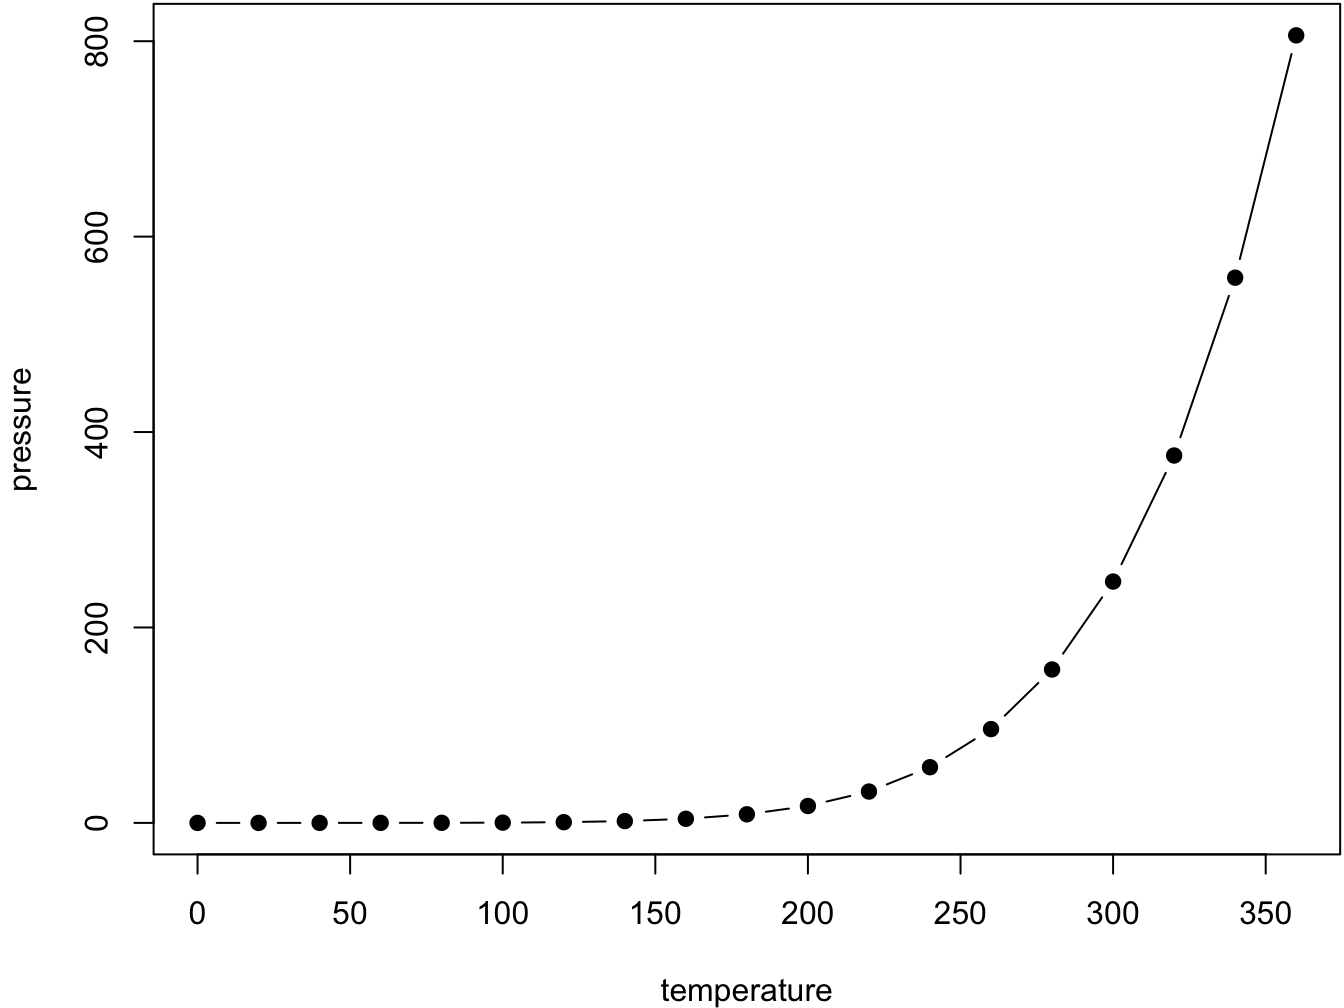
\includegraphics[width=0.8\linewidth]{methods_comp_book_files/figure-latex/nice-fig-1} 

}

\caption{Here is a nice figure!}\label{fig:nice-fig}
\end{figure}

Reference a figure by its code chunk label with the \texttt{fig:}
prefix, e.g., see Figure \ref{fig:nice-fig}. Similarly, you can
reference tables generated from \texttt{knitr::kable()}, e.g., see Table
\ref{tab:nice-tab}.

\begin{Shaded}
\begin{Highlighting}[]
\NormalTok{knitr}\OperatorTok{::}\KeywordTok{kable}\NormalTok{(}
  \KeywordTok{head}\NormalTok{(iris, }\DecValTok{20}\NormalTok{), }\DataTypeTok{caption =} \StringTok{'Here is a nice table!'}\NormalTok{,}
  \DataTypeTok{booktabs =} \OtherTok{TRUE}
\NormalTok{)}
\end{Highlighting}
\end{Shaded}

\begin{table}[t]

\caption{\label{tab:nice-tab}Here is a nice table!}
\centering
\begin{tabular}{rrrrl}
\toprule
Sepal.Length & Sepal.Width & Petal.Length & Petal.Width & Species\\
\midrule
5.1 & 3.5 & 1.4 & 0.2 & setosa\\
4.9 & 3.0 & 1.4 & 0.2 & setosa\\
4.7 & 3.2 & 1.3 & 0.2 & setosa\\
4.6 & 3.1 & 1.5 & 0.2 & setosa\\
5.0 & 3.6 & 1.4 & 0.2 & setosa\\
\addlinespace
5.4 & 3.9 & 1.7 & 0.4 & setosa\\
4.6 & 3.4 & 1.4 & 0.3 & setosa\\
5.0 & 3.4 & 1.5 & 0.2 & setosa\\
4.4 & 2.9 & 1.4 & 0.2 & setosa\\
4.9 & 3.1 & 1.5 & 0.1 & setosa\\
\addlinespace
5.4 & 3.7 & 1.5 & 0.2 & setosa\\
4.8 & 3.4 & 1.6 & 0.2 & setosa\\
4.8 & 3.0 & 1.4 & 0.1 & setosa\\
4.3 & 3.0 & 1.1 & 0.1 & setosa\\
5.8 & 4.0 & 1.2 & 0.2 & setosa\\
\addlinespace
5.7 & 4.4 & 1.5 & 0.4 & setosa\\
5.4 & 3.9 & 1.3 & 0.4 & setosa\\
5.1 & 3.5 & 1.4 & 0.3 & setosa\\
5.7 & 3.8 & 1.7 & 0.3 & setosa\\
5.1 & 3.8 & 1.5 & 0.3 & setosa\\
\bottomrule
\end{tabular}
\end{table}

You can write citations, too. For example, we are using the
\textbf{bookdown} package \citep{R-bookdown} in this sample book, which
was built on top of R Markdown and \textbf{knitr} \citep{xie2015}.

\chapter{Multi Level Modeling}\label{multi-level-modeling}

\section{Background}\label{background}

Multilevel data most frequently contains observations that are nested
within larger spatial categories or groupings (individuals within a
country) (Jones 2010). Can also contain observations that are nested
temporally (annual GDP) and may even be nested in larger spatial
groupings, across time (individual responses within surveys within
years). The beauty of multilevel modeling is that it does not lose the
information that will happen when you pool the information or use
techniques like fixed effects (Achen 2005).

\subsection{How to Deal with Multilevel
Data}\label{how-to-deal-with-multilevel-data}

Disaggregate group data to individual level: for example, individual
data nested within states, include state level variables at individual
level with same values for all individuals in a given state. PROBLEM:
all unmodeled contextual information (usually macro effects) ends up in
the error term. Individuals within same macro group then have correlated
errors (violating OLS assumption).

Pooling: when you assume there is not heterogeneity among the units (so
that people in U.S. are similar to people in Canada, Mexico, New
Zealand, China, and Nigeria). If you are assuming this, then you can use
a garden variety regression (Jones 2010). However, this assumption will
likely be incorrect (Franzese 2005). If incorrect, then you likely
introduce heteroskedasticity as well as autocorrelation (this mainly
occurs because respondents, \(i\), in U.S. will be more alike to each
other than respondents in New Zealand (Jones 2010; Priomo ea 2007). This
will lead to inefficient and inconsistent standard errors leading to
invalid hypothesis testing (Jones 2010). If you are only afraid of
non-spherical errors, then you can use what is commonly referred to as
the ``Huber-White sandwich'' estimator (White 1980; Jones 2010; Primo ea
2007). However, much of the information that we care about is lost if we
don't use multilevel modeling.

Solutions:

\begin{itemize}
\tightlist
\item
  Fixed effects (not very common in political science): Essentially
  adding an additional dummy variable for each macro-level groupings to
  account for contextual variation. It is shown with the following
  equation: \(y_i = \beta_{j[I]} + \beta_1x_i + \epsilon_i\).where
  \(\beta_j\) gives a different intercept for each unit. Prevents
  correlated error issue, but will be inefficient given that we burn a
  degree of freedom for every new independent variable we are adding to
  the model. Additionally, all covariates that are constant within \(j\)
  cannot be estimated (Jones 2010). A variation of the fixed effect is
  to estimate a model for each unit and then compare the different
  coefficients, however the unbalanced nature of political science data
  commonly precludes this kind of analysis or at least makes some
  estimates will wide variability that has nothing to do with theory and
  everything to do with sample size (Jones 2010).
\item
  Random effects (not very common in political science): like fixed
  effects, allows the estimation of different intercepts for each
  macro-level group. The formula for this one is
  \(y_i = \beta_{j[I]} + \epsilon_i\). The difference between fixed and
  random effects is the way \(\beta_{j[I]}\) is treated. Under fixed
  effects, the unit effects are unknown constants that are estimated
  from the data (Faraway 2006). This approach treats it as a random
  coefficient by assuming these intercepts are randomly drawn for a
  given (usually normal) distribution (Gelman and Hill 2007). However,
  estimates may be biased.
\item
  Clustering (much more common but kind of like a band-aid): essentially
  a statistical ``fix'' of the problem by allowing a compound error term
  that accounts for the macro-level information. It is a variation of
  the Huber-White robust standard error. Cluster-adjustment works well
  for procedures including logit and probit assuming that the number of
  clusters is large enough. Simulations have shown that 50 clusters are
  more than sufficient (Kezdi 2003).
\item
  Multilevel Modeling (probably theoretically better, but not
  necessarily methodologically): Also known as Hierarchical Linear
  Modeling or Mixed Effects Modeling. Commonly used in education
  research (students within classes, within schools, within school
  districts, etc). Goal is to predict influences on a dependent variable
  using independent variables from several contexts (individual and
  macro). I think the equation looks like this:
  \(y_i = \beta_0 + \beta_1x_i + \beta_2z_j + \epsilon_i\) where the
  \(x\) is the level 1 data and \(z\) is the level 2 data.
\end{itemize}

\section{Assumptions}\label{assumptions}

Not so much an assumption, but you should have a lot more observations
in the first stage than in the second stage (Achen 2005). However,
having a small number of observations at the second level, we open
ourselves up to bias and incorrect hypothesis testing (if the
distributional assumptions are off (Bowers and Drake 2005)). Bowers and
Drake (2005) suggest using graphs of the differences between second
level groups to check assumptions. Additionally, hierarchical models are
delicate meaning that specification error in the first stage will lead
to biases and inconsistencies at the second stage, even if the second
stage is properly handled (Achen 2005).

\section{Estimating Multilevel
Modeling}\label{estimating-multilevel-modeling}

For multilevel modeling:

Level 1: \(y_{ij} = \alpha_{j[i]} + \beta x_i + \epsilon_i\)

Level 2: \(\alpha_j ~ N(\mu_\alpha,\sigma^2_\alpha)\) or
\(\alpha_j = \gamma_0 + \gamma_1u_j + \eta_j\)

Where: i = individuals, j = groups

Considerations for Multilevel modeling:

\begin{itemize}
\tightlist
\item
  How many levels are in the data? - Social science generally only has 2
  or 3
\item
  How many predictors for each level are needed? - Modeling becomes
  increasingly complex as these increase (especially for macro-level
  predictors). Are any cross-level interactions hypothesized? Which
  parts of the model will include random effects? What structural form
  will you use? -Varying intercepts only, varying slopes only, varying
  intercepts and slopes.

  \begin{itemize}
  \tightlist
  \item
    Varying intercepts: will have same slope, but cross y-axis at
    different places.\\
  \item
    Varying slopes: will have same intercept, but different slopes
  \item
    Varying slopes and intercepts: will have both
  \end{itemize}
\end{itemize}

If you choose varying intercept and slope, you add additional layer of
complexity. Level 1 stays the same, but level 2 now has to account for
fact that the intercept and slope will vary.

\section{Additional Considerations for Multilevel
Modeling}\label{additional-considerations-for-multilevel-modeling}

Number of groups: Some argue that a minimum number of groups is needed
for multilevel modeling. However, even with a small number of groups, a
multilevel regression will simply reduce to a classical regression.
Therefore, the number of groups is a limitation, only in that the
estimation of between-group variation will be limited.

Number of observations per group: Another issue that is brought up, but
doesn't really exist. With small numbers of observations in some groups,
estimates of the \(\alpha\) parameters for those groups will be
imprecise. Also, if there is significant imbalance there can be issues
with random effects estimates.

\chapter{Methods}\label{methods}

We describe our methods in this chapter.

\chapter{Applications}\label{applications}

Some \emph{significant} applications are demonstrated in this chapter.

\section{Example one}\label{example-one}

\section{Example two}\label{example-two}

\chapter{Final Words}\label{final-words}

We have finished a nice book.

\bibliography{book.bib,packages.bib}


\end{document}
